% Created 2022-07-10 Sun 10:32
% Intended LaTeX compiler: pdflatex
\documentclass[presentation,mathserif,table]{beamer}
\usepackage[utf8]{inputenc}
\usepackage[T1]{fontenc}
\usepackage{graphicx}
\usepackage{grffile}
\usepackage{longtable}
\usepackage{wrapfig}
\usepackage{rotating}
\usepackage[normalem]{ulem}
\usepackage{amsmath}
\usepackage{textcomp}
\usepackage{amssymb}
\usepackage{capt-of}
\usepackage{hyperref}
\usepackage{minted}
\beamertemplatenavigationsymbolsempty
\usepackage[T1]{fontenc}
\usepackage{DejaVuSans}
\usepackage{DejaVuSansMono}
\usefonttheme{professionalfonts}
\usepackage[euler-digits,euler-hat-accent]{eulervm}
\setbeamertemplate{itemize items}{•}
\setbeamertemplate{enumerate items}[default]
\AtBeginSection[]
{
\begin{frame}<beamer>
\frametitle{Outline}
\tableofcontents[currentsection]
\end{frame}
}
\setcounter{tocdepth}{1}
\setbeamertemplate{headline}{}
\setbeamertemplate{footline}{
\leavevmode%
\hbox{%
\begin{beamercolorbox}[wd=\paperwidth,ht=2.25ex,dp=1ex,right]{fg=black}%
\usebeamerfont{section in head/foot}\insertsection\hspace*{2em}
\insertframenumber{} / \inserttotalframenumber\hspace*{2ex}
\end{beamercolorbox}%
}%
\vskip0pt%
}
\usepackage{appendixnumberbeamer}
\setbeamersize{text margin left=3mm,text margin right=3mm}
\newcommand\blfootnote[1]{%
\begingroup
\renewcommand\thefootnote{}\footnote{#1}%
\addtocounter{footnote}{-1}%
\endgroup
}
\setbeamerfont{footnote}{size=\tiny}
\usepackage{tikz}
\usepackage[retainorgcmds]{IEEEtrantools}
\hypersetup{colorlinks=true, allcolors=., urlcolor=blue}
\usepackage[absolute,overlay]{textpos}
\usepackage{xcolor}
\definecolor{LightGray}{gray}{0.96}
\usepackage{minted}
\setminted{bgcolor=LightGray, fontsize=\small}
\newcommand{\eg}{e.g.\,}
\newcommand{\ie}{i.e.\,}
\newcommand{\aka}{a.k.a.\,}
\newcommand{\etc}{\emph{etc.}\,}
\newcommand{\X}{{\mathbold X}}
\newcommand{\bS}{{\mathbold S}}
\newcommand{\bSigma}{{\mathbold \Sigma}}
\newcommand{\x}{{\mathbold x}}
\newcommand{\bbeta}{{\mathbold \beta}}
\newcommand{\Y}{{\mathbold Y}}
\newcommand{\y}{{\mathbold y}}
\newcommand{\B}{{\mathbold B}}
\newcommand{\W}{{\mathbold W}}
\newcommand{\U}{{\mathbold U}}
\newcommand{\V}{{\mathbold V}}
\newcommand{\bH}{{\mathbold H}}
\newcommand{\R}{\mathbb{R}}
\DeclareMathOperator*{\argmin}{argmin}
\DeclareMathOperator*{\argmax}{argmax}
\DeclareMathOperator*{\tv}{TV}
\DeclareMathOperator*{\Tr}{Tr}
\DeclareMathOperator*{\FFT}{FFT}
\DeclareMathOperator*{\IFFT}{IFFT}
\DeclareMathOperator*{\diag}{diag}
\DeclareMathOperator*{\supp}{supp}
\DeclareMathOperator*{\tf}{tf}
\DeclareMathOperator*{\idf}{idf}
\DeclareMathOperator*{\df}{df}
\DeclareMathOperator*{\Var}{Var}
\DeclareMathOperator*{\Frob}{Frob}
\DeclareMathOperator*{\F}{F}
\DeclareMathOperator*{\softmax}{softmax}
\DeclareMathOperator*{\AUC}{AUC}
\usepackage{bm}
\usecolortheme{dove}
\setbeamercolor*{block title example}{fg=black,bg=white}
\setbeamercolor*{block body example}{fg=black,bg=white}
\usetheme{default}
\author{Jerome Dockes}
\date{}
\title{Machine learning Part 2}
\author{Jérôme Dockès \& Nikhil Bhagwat}
\titlegraphic{
\includegraphics[height=1.5cm]{figures/mcgill-university.png} \hspace{1.5cm} 
\includegraphics[height=1.5cm]{figures/origami-lab-logo.png}}
\date{QLS612 course 2022-07-12}
\subtitle{Model selection \& validation}
\hypersetup{
 pdfauthor={Jerome Dockes},
 pdftitle={Machine learning Part 2},
 pdfkeywords={},
 pdfsubject={},
 pdfcreator={Emacs 26.3 (Org mode 9.3.7)}, 
 pdflang={English}}
\begin{document}

\maketitle
\section{Introduction: cross-validation}
\label{sec:org5c992e6}
\subsection{Recap of part 1}
\label{sec:org057d5e5}
\begin{frame}[label={sec:org6c1ae67}]{Recap of part 1}
\begin{block}{Supervised learning}
\begin{itemize}
\item Regression: least-squares linear regression
\item Classification: logistic regression
\end{itemize}
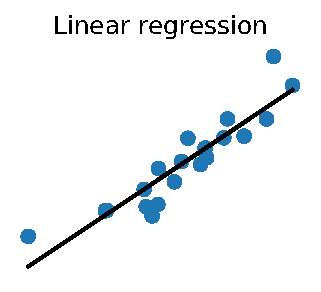
\includegraphics[height=.4 \textheight]{figures/generated/linear_regression_1d/linear_regression.pdf}
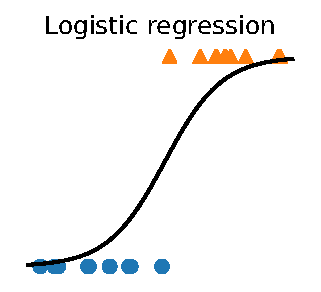
\includegraphics[height=.4 \textheight]{figures/generated/logistic_regression_1d/logistic_regression.pdf}
\end{block}
\end{frame}

\begin{frame}[label={sec:orgae44545}]{Recap of part 1}
\begin{block}<1->{Supervised learning}
\begin{itemize}
\item Regression: least-squares linear regression
\item Classification: logistic regression
\end{itemize}
\end{block}
\begin{block}<1->{Regularization}
\begin{itemize}
\item \(\ell_2\) \aka ridge regularization
\end{itemize}
\end{block}
\begin{block}<2->{Model evaluation and selection}
\begin{itemize}
\item Out-of-sample generalization; independent test set
\item Performance metrics:
\begin{itemize}
\item regression: mean squared error
\item classification: accuracy, ROC curve
\end{itemize}
\item Cross-validation
\end{itemize}
\end{block}
\end{frame}
\begin{frame}[label={sec:orgc5197aa}]{Notation \& vocabulary}
\begin{block}{Supervised learning framework}
\begin{equation}
Y = f(X) + E
\end{equation}
\vspace{-10pt}
\begin{itemize}[<+->]
\item \(Y \in \R\): output (\aka target, dependent variable) to predict
\item \(X \in \R^p\): features (\aka inputs, regressors, descriptors, independent variables)
\item \(E \in \R\): unmodelled noise
\item \(f\): the function we try to approximate
\end{itemize}
\end{block}
\begin{block}<4->{Example: linear regression}
\vspace{-20pt}
 \begin{IEEEeqnarray}{rCl}
 Y & = & \beta_0 + \langle X, \beta \rangle + E \\
& = & \beta_0 + \sum_{j=1}^p X_j \, \beta_j + E
 \end{IEEEeqnarray}
"learning" = choosing \(\beta_0 \in \R\) and \(\bbeta \in \R^p\)
\end{block}
\end{frame}
\begin{frame}[label={sec:org6390761}]{How to set parameters: Empirical Risk Minimization}
\begin{itemize}
\item Choose a loss function \(L\) measuring how bad is our error.
\item Example: squared error \(L(Y, \hat{Y}) = (Y - \hat{Y})^2\), where \(\hat{Y}\) is the prediction
\item We want to minimize the expected error (risk): \(\mathbb{E}[L(Y, \hat{Y})]\)
\end{itemize}
\end{frame}
\begin{frame}[label={sec:orgf7932d1}]{How to set parameters: Empirical Risk Minimization}
We do not know the risk: estimate it from a sample.

Given \(n\) training examples \(\X \in \R^{n \times p}\), \(\y \in \R^n\),
minimize the empirical risk: \(\sum_{i=1}^n L(\y_i, \hat{\y_i})\)

\begin{block}{For linear regression:}
find \(\hat{\beta}_0 \in \R, \hat{\bbeta} \in \R^p\) that minimize
\begin{IEEEeqnarray}{rcl}
\| \y - \hat{\y} \|_2^2 & \; = \; & \| \y - \hat{\beta}_0 - \X \, \hat{\bbeta} \|_2^2 \\
& \; = \; & \sum_{i=1}^n (\y_i - \hat{\beta}_0 - \sum_{j=1}^p \X_{ij}\, \hat{\bbeta}_j )^2
\end{IEEEeqnarray}

"Fitting" the parameters to \(\X, \y\).
\end{block}
\end{frame}

\begin{frame}[label={sec:org3cddaf0}]{Evaluating a model}
\begin{block}{We always want to do 2 distinct things:}
\begin{itemize}
\item Select a model.
\item Evaluate its performance.
\end{itemize}

\vfill
\end{block}

\begin{structureenv} %% warning
We can never do both on the same data!
\end{structureenv}
\end{frame}
\begin{frame}[label={sec:orgbd65493}]{Training error is a biased estimator of the risk}
\begin{itemize}
\item 30 different models (eg 30 possible values for \(\hat{\beta}_0, \hat{\bbeta}\))
\item All have a risk (expected accuracy) of 0.5
\item Evaluate on a first dataset
\end{itemize}
\begin{center}
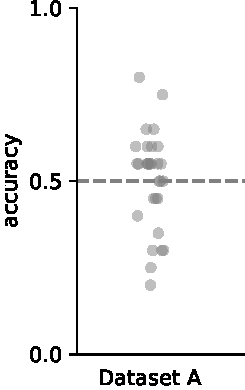
\includegraphics[height=.5 \textheight]{figures/generated/select_evaluate/select_evaluate_1.pdf}
\end{center}
\end{frame}
\begin{frame}[label={sec:org9858780}]{Training error is a biased estimator of the risk}
\begin{itemize}
\item 30 different models (eg 30 possible values for \(\hat{\beta}_0, \hat{\bbeta}\))
\item All have a risk (expected accuracy) of 0.5
\item Evaluate on a first dataset \alert{\alert{and select the best model}}
\end{itemize}
\begin{center}
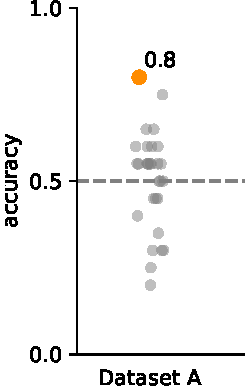
\includegraphics[height=.5 \textheight]{figures/generated/select_evaluate/select_evaluate_2.pdf}
\end{center}
\end{frame}
\begin{frame}[label={sec:org017d8fc}]{Training error is a biased estimator of the risk}
On a new dataset, the selected model will perform on average:
\begin{enumerate}
\item Better than on dataset A?
\item Worse than on dataset A?
\item The same?
\end{enumerate}
\begin{center}
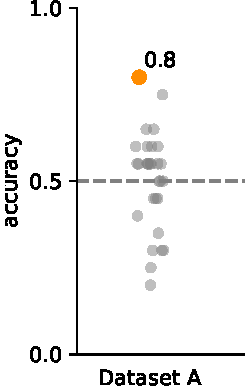
\includegraphics[height=.5 \textheight]{figures/generated/select_evaluate/select_evaluate_2.pdf}
\end{center}
\end{frame}

\begin{frame}[label={sec:org4f15e9d}]{Training error is a biased estimator of the risk}
The selected model is more likely to perform worse on average than on dataset A.
\begin{center}
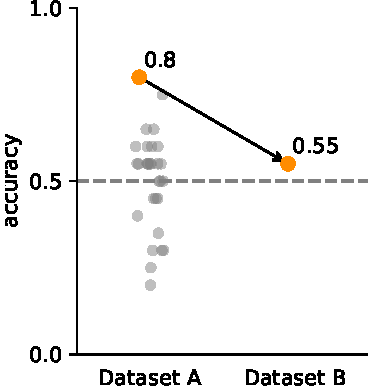
\includegraphics[height=.5 \textheight]{figures/generated/select_evaluate/select_evaluate_3.pdf}
\end{center}
\end{frame}
\begin{frame}[label={sec:org6d70d0c}]{Training error is a biased estimator of the risk}
The selected model is more likely to perform worse on average than on the dataset used to select it:

To estimate its risk we need a new dataset.
\begin{center}
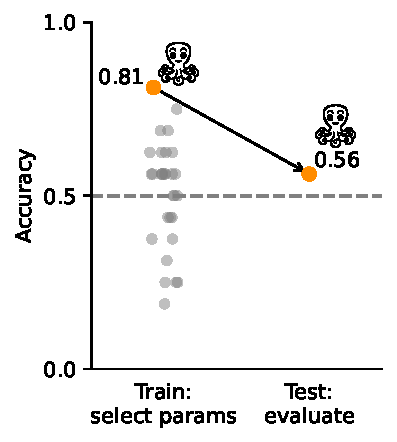
\includegraphics[height=.5 \textheight]{figures/generated/select_evaluate/select_evaluate_4.pdf}
\end{center}
\end{frame}

\begin{frame}[label={sec:orgc3feb19}]{Training error is a biased estimator of the risk}
Distribution of train and test errors across 30 experiments:
\begin{center}
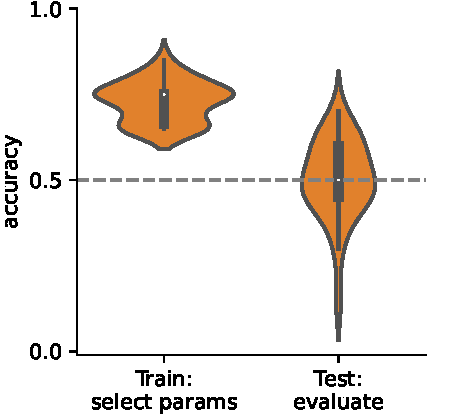
\includegraphics[height=.5 \textheight]{figures/generated/select_evaluate_averaged/select_evaluate_averaged_1.pdf}
\end{center}
\end{frame}
\begin{frame}[label={sec:org7f42933}]{Training error is a biased estimator of the risk}
\begin{itemize}
\item The systematic difference is the bias.
\item It is why we cannot use the training error to estimate model performance.
\end{itemize}
\begin{center}
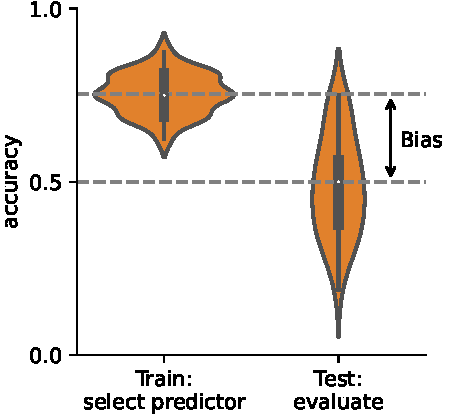
\includegraphics[height=.5 \textheight]{figures/generated/select_evaluate_averaged/select_evaluate_averaged_2.pdf}
\end{center}
\end{frame}


\begin{frame}[label={sec:org7fb7314}]{Estimating prediction performance}
When you hear "best", "maximum", "select", \ldots{} think "bias"
\begin{block}{Setting the parameters}
\begin{itemize}
\item \alert{Select} \(\bbeta\) that gives the \alert{best} prediction on training data
\item The prediction score for \(\hat{\bbeta}\) is biased: compute a new score on unseen test data.
\end{itemize}
\end{block}
\end{frame}
\subsection{Supervised learning with sklearn}
\label{sec:org4bda54a}
\begin{frame}[label={sec:orge4c7180},fragile]{scikit-learn "estimator API": \texttt{fit; predict}}
 \begin{minted}[]{python}
estimator = Ridge()
estimator.fit(X_train, y_train)
predictions = estimator.predict(X_test)
\end{minted}
\vfill
\href{https://scikit-learn.org/stable/getting\_started.html}{Scikit-learn user guide}

\href{https://scikit-learn.org/stable/modules/generated/sklearn.linear\_model.Ridge.html}{\texttt{sklearn.linear\_model.Ridge}}
\end{frame}

\begin{frame}[label={sec:orge9ce74a},fragile]{Evaluating performance with \texttt{sklearn.metrics}}
 \begin{minted}[]{python}
estimator = Ridge()
estimator.fit(X_train, y_train)
predictions = estimator.predict(X_test)

mse = metrics.mean_squared_error(y_test, predictions)
\end{minted}
\vfill

\href{https://scikit-learn.org/stable/modules/generated/sklearn.linear\_model.Ridge.html}{\texttt{sklearn.linear\_model.Ridge}}

\href{https://scikit-learn.org/stable/modules/classes.html\#module-sklearn.metrics}{\texttt{sklearn.metrics}}

\href{https://scikit-learn.org/stable/modules/model\_evaluation.html}{User guide on model evaluation}
\vfill
\texttt{ex\_01\_fit\_predict\_questions.py}
\end{frame}

\subsection{cv}
\label{sec:orgd9ca64b}
\begin{frame}[label={sec:org3dc3c30},fragile]{Cross-validation}
 \begin{center}
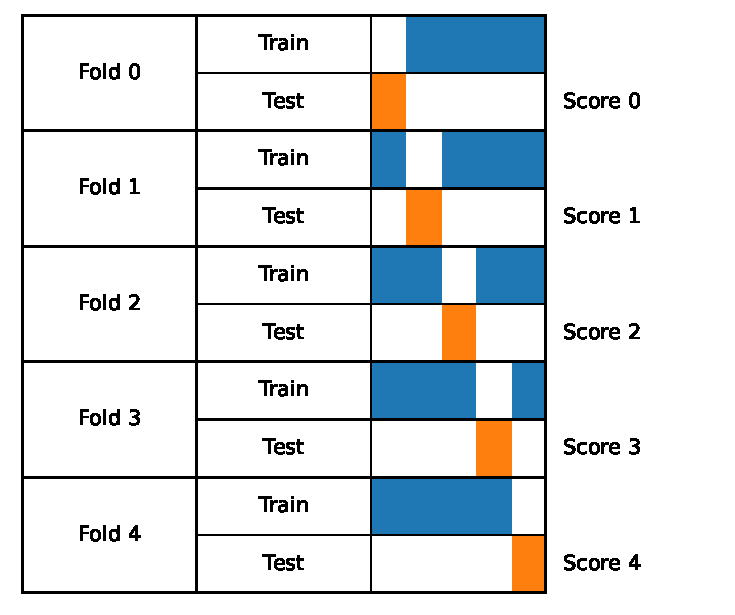
\includegraphics[height=.7 \textheight]{figures/generated/cv_figure_simple.pdf}
\end{center}

\href{https://scikit-learn.org/stable/modules/cross\_validation.html}{\texttt{scikit-learn.org/stable/modules/cross\_validation.html}}
\href{https://scikit-learn.org/stable/modules/generated/sklearn.model\_selection.GridSearchCV.html}{\texttt{sklearn.model\_selection.cross\_validate}}

\texttt{ex\_02\_cross\_validate\_questions.py}
\end{frame}
\section{Model and hyperparameter selection}
\label{sec:orge495433}
\subsection{nested cv}
\label{sec:orgee48f5e}

\begin{frame}[label={sec:org7cc4cc3}]{Need for regularization}
Linear regression: projection on the column space of \(X\)
\vspace{10pt}
\begin{structureenv} %% top
\begin{columns}
\begin{column}{.3\columnwidth}
\begin{equation}
\hat{\y} = \X \, \hat{\bbeta}
\end{equation}
\end{column}

\begin{column}{.7\columnwidth}
\vspace{-17pt}
\begin{center}
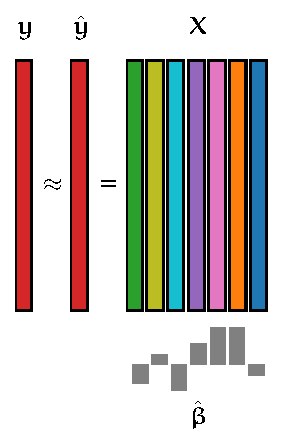
\includegraphics[height=.7\textheight]{figures/generated/dim_reduction_colors/regression_full_3.pdf}
\end{center}
\end{column}
\end{columns}
\end{structureenv}

\begin{structureenv} %% bottom
\begin{itemize}
\item Too many features: high variance \& unstable solution
\item Solutions: regularization, dimensionality reduction
\end{itemize}
\end{structureenv}
\end{frame}
\begin{frame}[label={sec:org9670e64}]{Regularization}
\begin{block}{Example: ridge regression}
\begin{equation}
\argmin_{\bbeta, \beta_0} \| \y - \beta_0 - \X \, \bbeta \|_2^2 + \alpha \, \|\bbeta\|_2^2
\end{equation}
\end{block}
\end{frame}
\begin{frame}[label={sec:org53e86e9}]{}
\begin{columns}
\begin{column}{.33\columnwidth}
\(\small{ \text{Var}(\hat{\beta}_i) = \mathbb{E}(\hat{\beta}_i  - \mathbb{E}(\hat{\beta}_i))^2}\)
\end{column}

\begin{column}{.38\columnwidth}
\vspace{-15pt}
\begin{center}
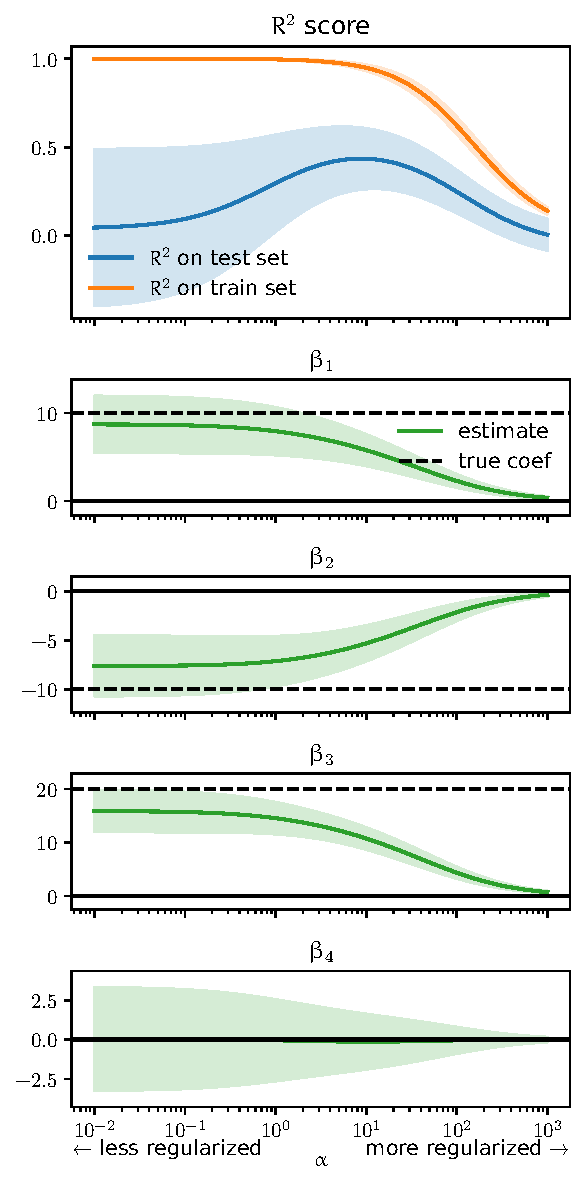
\includegraphics[height=\textheight]{figures/generated/ridge_regularization_path/ridge_regularization_path.pdf}
\end{center}
\end{column}
\begin{column}{.3\columnwidth}
\(\small \text{Bias}(\hat{\beta}_i) = \mathbb{E}(\hat{\beta}_i) - \beta_i\)
\end{column}
\end{columns}
\end{frame}

\begin{frame}[label={sec:orge733eff}]{Setting hyperparameters}
\begin{block}{How can we choose the ridge hyperparameter \(\alpha\)?}
\end{block}
Try a few and pick the best one\ldots{}

But measure its performance on separate data!
\end{frame}
\begin{frame}[label={sec:org064b835}]{Nested cross-validation}
When you hear "best", "maximum", "select", \ldots{} think "bias"
\begin{block}<2->{Setting the parameters}
\begin{itemize}
\item \alert{Select} \(\bbeta\) that gives the \alert{best} prediction on training data
\item The prediction score for \(\hat{\bbeta}\) is biased: compute a new score on unseen test data.
\end{itemize}
\end{block}
\begin{block}<3->{Setting the hyperparameters}
\begin{itemize}
\item Repeat step 1 for a few values of \(\alpha\), fitting and testing several models
\item \alert{Select} the hyperparameter that obtains the \alert{best} prediction on test data
\item The prediction score of that model on \emph{test} data is biased: evaluate it again on unseen data
\end{itemize}
\end{block}
\end{frame}
\begin{frame}[label={sec:org5afbcda}]{One split}
\begin{center}
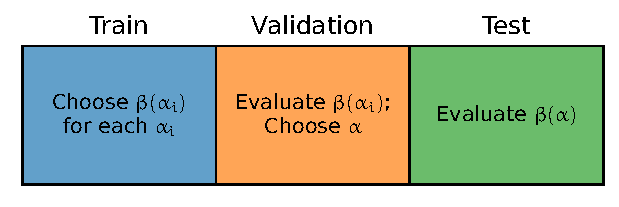
\includegraphics[width=.9\linewidth]{figures/generated/train_eval_test/datasets.pdf}
\end{center}
\end{frame}
\begin{frame}[label={sec:org965b05e},fragile]{Nested cross-validation}
 \begin{center}
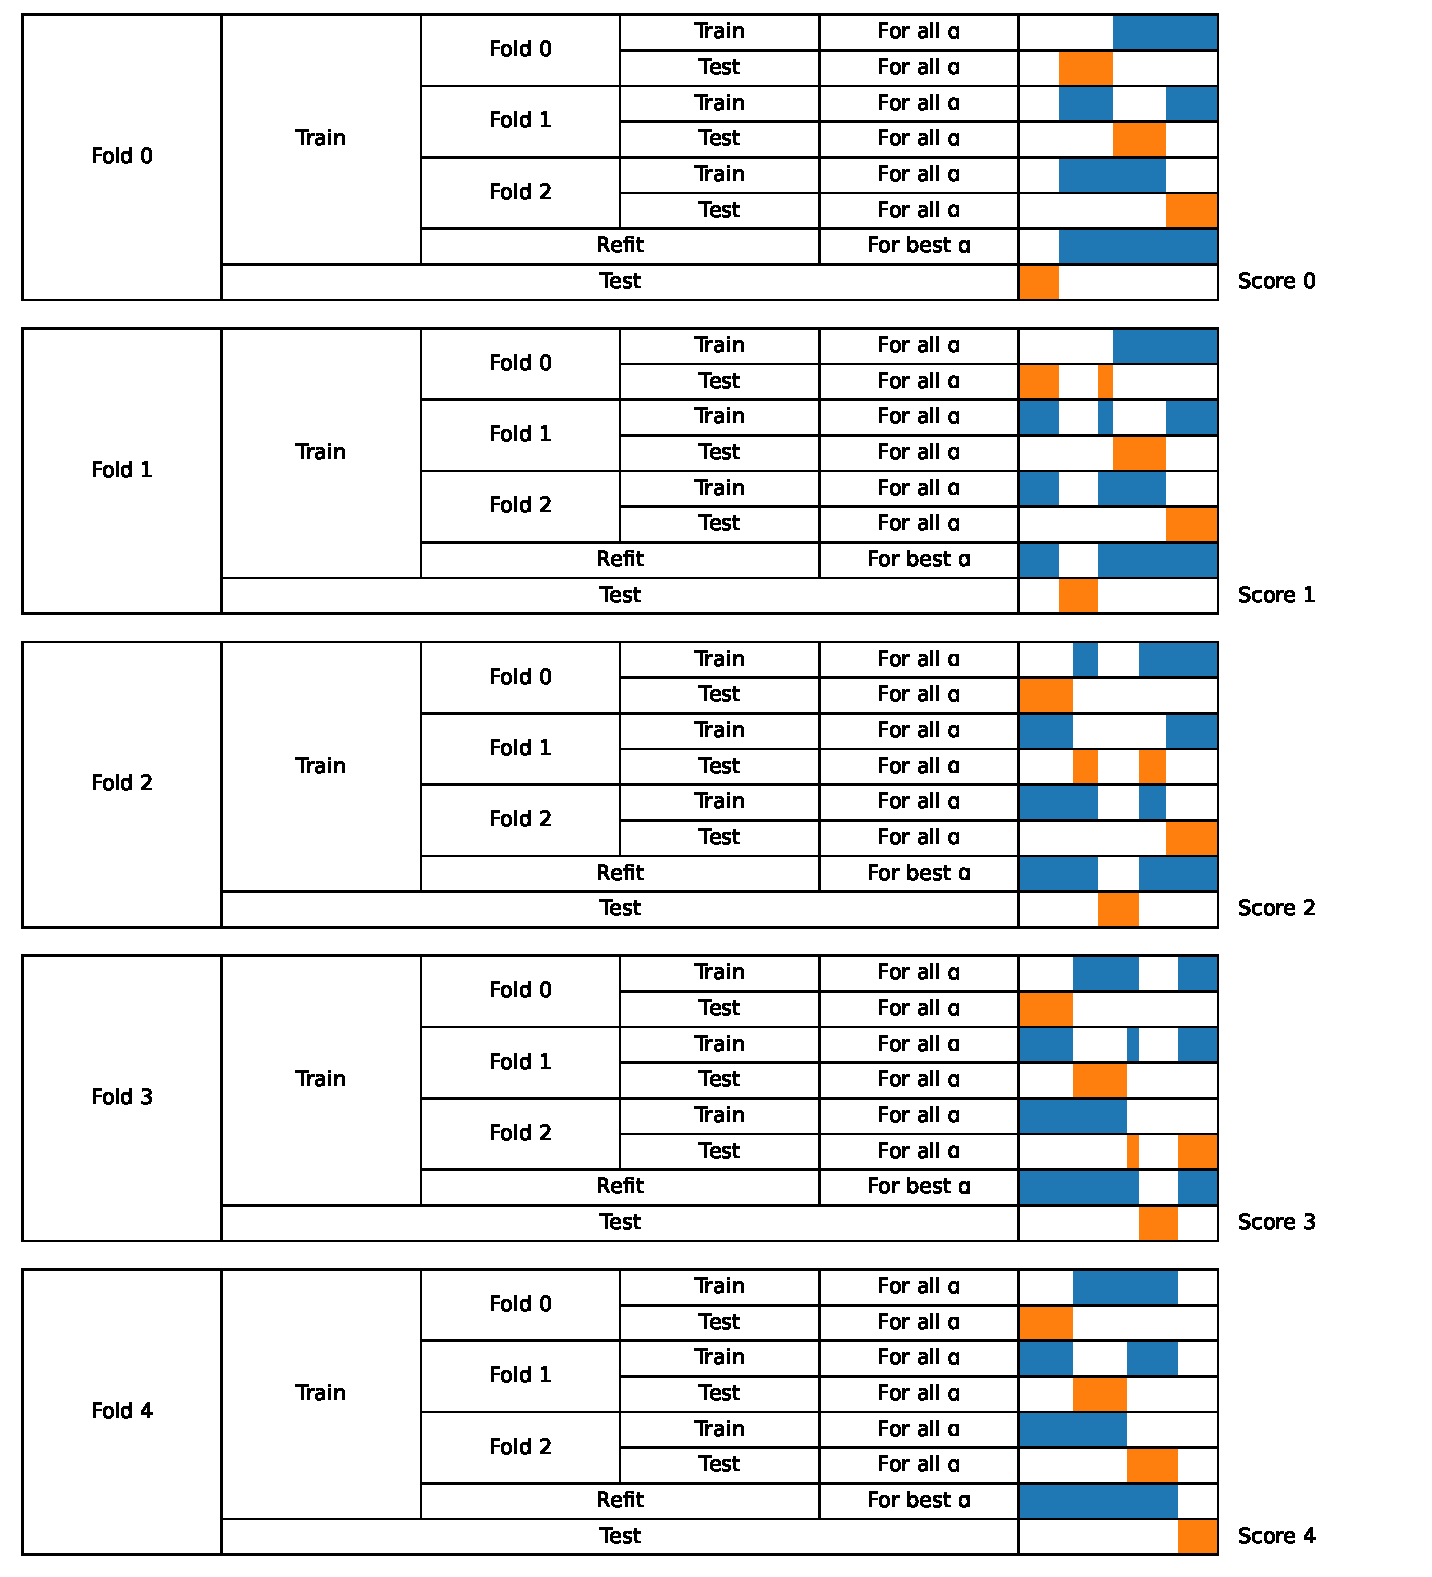
\includegraphics[width=.9\linewidth]{figures/generated/cv_figure_nested.pdf}
\end{center}
  see  \href{https://scikit-learn.org/stable/modules/generated/sklearn.model\_selection.GridSearchCV.html}{\texttt{sklearn.model\_selection.GridSearchCV}}
\end{frame}

\begin{frame}[label={sec:orge888e9e},fragile]{Nested cross-validation with scikit-learn}
 \begin{itemize}
\item In general: \href{https://scikit-learn.org/stable/modules/generated/sklearn.model\_selection.GridSearchCV.html}{\texttt{GridSearchCV}} (\href{https://scikit-learn.org/stable/modules/grid\_search.html\#grid-search}{User Guide})
\end{itemize}
\vfill
\begin{minted}[]{python}
model = GridSearchCV(
    Ridge(), {"alpha": [.1, 1., 10.]})
scores = cross_validate(model, X, y)["test_score"]
\end{minted}
\vfill
\begin{itemize}
\item Use \href{https://scikit-learn.org/stable/glossary.html\#term-cross-validation-estimator}{CV estimators} when possible: \href{https://scikit-learn.org/stable/modules/generated/sklearn.linear\_model.RidgeCV.html}{\texttt{RidgeCV}}, \href{https://scikit-learn.org/stable/modules/generated/sklearn.linear\_model.LassoCV.html}{\texttt{LassoCV}}, \ldots{}
\end{itemize}

\vfill

\texttt{ex\_03\_grid\_search\_regression\_questions.py}
\end{frame}
\begin{frame}[label={sec:orgf98d88b},fragile]{Implementing nested CV}
 \texttt{ex\_04\_nested\_cross\_validation\_questions.py}
\end{frame}
\section{Dimensionality reduction}
\label{sec:org5580bbe}
\subsection{Intro}
\label{sec:org47316d1}
\begin{frame}[label={sec:org77e487e}]{Dimensionality reduction}
\begin{equation}
\hat{\y} = \hat{\beta}_0 + \hat{\bbeta}_1 \, \X_{:, 1} + \hat{\bbeta}_2 \, \X_{:, 1} + \dots + \hat{\bbeta}_p \, \X_{:, p}
\end{equation}
\begin{block}{Problems when the number of features \(p\) becomes large}
\begin{itemize}
\item Bigger errors on test data (larger variance of predictions)
\item Numerical stability issues
\item Computational cost and memory usage
\end{itemize}
\end{block}
\end{frame}
\begin{frame}[label={sec:orgfeb4409}]{Dimensionality reduction}
\begin{block}{Until now}
\begin{center}
\includegraphics[height=.12 \textheight]{figures/graphs/pipeline-1.pdf}
\end{center}
\end{block}
\begin{block}{Add a step in the pipeline: simplifying the inputs}
\begin{center}
\includegraphics[height=.12 \textheight]{figures/graphs/pipeline-2.pdf}
\end{center}
\end{block}
\end{frame}
\begin{frame}[label={sec:org99111e2},fragile]{Simulated data for linear regression}
 \begin{itemize}
\item Generate \(\X \in \R^{n \times 3}\), \(\mathbold{\bbeta} \in \R^3\), \(\mathbold{e} \in \R^n\) and \(\y = \X \, \bbeta + \mathbold{e} \in R^n\)
\item Append columns containing random noise to \(\X\)
\item Now \(\X \in \R^{n \times p}\), with \(p \geq 3\), but only the first 3 columns are linked with \(\y\)
\item Split into training and testing tests and evaluate a linear regression model: what happens when \(p\) becomes large?
\end{itemize}

See \href{https://scikit-learn.org/stable/modules/generated/sklearn.datasets.make\_regression.html\#sklearn.datasets.make\_regression}{\texttt{sklearn.datasets.make\_regression}} for generating data
\begin{center}
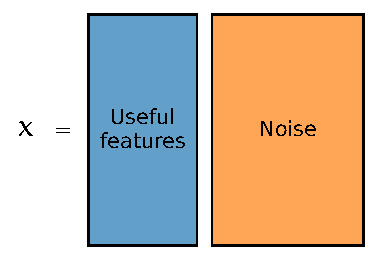
\includegraphics[height=.4 \textheight]{figures/generated/show_make_regression/x_construction.pdf}
\end{center}
\end{frame}
\begin{frame}[label={sec:orga3c84af}]{Model complexity: overfitting}
\begin{itemize}
\item Model complexity increases with dimension.
\item Example: a linear model in dimension \(p\) can fit exactly (0 training error) any set of \(p + 1\) points.
\item Risk of overfitting: fitting exactly training data but failing on test data
\end{itemize}

\begin{center}
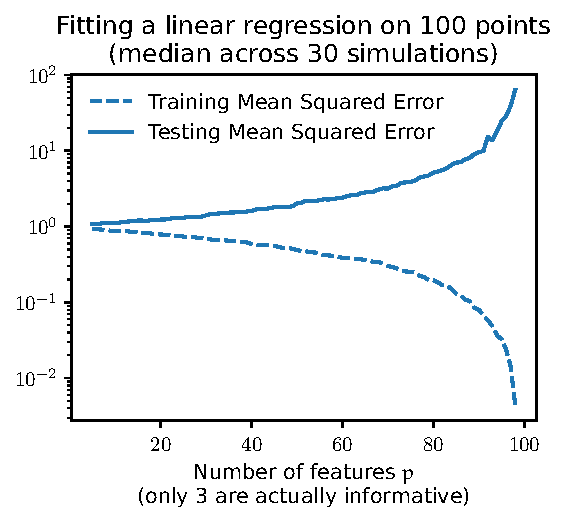
\includegraphics[height=.7\textheight]{figures/generated/ridge_overfitting/mse_log.pdf}
\end{center}
\end{frame}
\subsection{Univariate feature selection}
\label{sec:orgcbdc7ab}
\begin{frame}[label={sec:org1e21bc3}]{Univariate feature selection}
\begin{itemize}
\item \aka feature screening, filtering \ldots{}
\item Check features (columns of \(\X\)) one by one for association with the output \(\y\)
\item Keep only a fixed number or percentage of the features
\end{itemize}
\begin{block}{Simple (linear) association criteria}
\begin{itemize}
\item for regression: correlation
\item for classification: ANalysis Of VAriance
\end{itemize}
\end{block}
\begin{block}{Read more in the scikit-learn user guide}
\href{https://scikit-learn.org/stable/modules/feature\_selection.html\#feature-selection}{scikit-learn feature selection}
\end{block}
\end{frame}

\begin{frame}[label={sec:orgd4889e1}]{Univariate feature selection}
Keeping only the 10 best features (most correlated with \(\y\))
\begin{center}
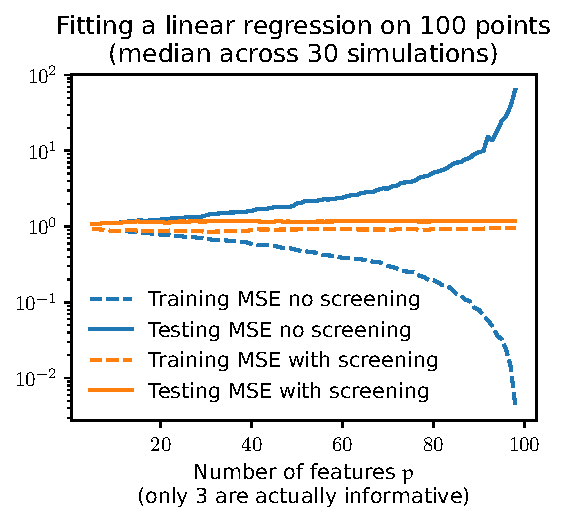
\includegraphics[height=.7\textheight]{figures/generated/ridge_overfitting/mse_with_dim_reduction_log.pdf}
\end{center}
\end{frame}

\subsection{Fit whole pipeline on train data only}
\label{sec:org87fb011}
\begin{frame}[label={sec:org98c07c6}]{Dataset transformations}
\begin{block}{Typical pipeline}
\begin{center}
\includegraphics[width=.9\linewidth]{figures/graphs/pipeline-2-no-color.pdf}
\end{center}
\end{block}
\begin{block}{Example}
\begin{center}
\includegraphics[width=.9\linewidth]{figures/graphs/pipeline-3.pdf}
\end{center}
\end{block}
\end{frame}
\begin{frame}[label={sec:org9bb7baf},fragile]{scikit-learn "transformer API": \texttt{fit; transform}}
 \begin{minted}[]{python}
transformer = SelectKBest()
transformer.fit(X_train)
transformed_train = transformer.transform(X_train)
\end{minted}
\begin{block}{can also be written:}
\begin{minted}[]{python}
transformer = SelectKBest()
transformed_train = transformer.fit_transform(X_train)
\end{minted}
\end{block}
\begin{structureenv} %% links
\vfill

\href{https://scikit-learn.org/stable/modules/feature\_selection.html}{scikit-learn feature selection}

\href{https://scikit-learn.org/stable/getting\_started.html\#transformers-and-pre-processors}{scikit-learn \texttt{Transformer} API}
  \vfill
\end{structureenv}
\end{frame}

\begin{frame}[label={sec:org72f4113},fragile]{\texttt{feature\_selection.SelectKBest}}
 \begin{block}{\texttt{fit:}}
\begin{itemize}
\item compute ANOVA or correlation for each column of \(X\)
\item Remember the indices of the \(k\) columns with highest scores
\end{itemize}
\end{block}
\begin{block}{\texttt{transform:}}
\begin{itemize}
\item Index input to keep only the \(k\) selected columns
\end{itemize}
\end{block}


\begin{structureenv} %% link
\href{https://scikit-learn.org/stable/modules/generated/sklearn.feature\_selection.SelectKBest.html\#sklearn.feature\_selection.SelectKBest}{\texttt{sklearn.feature\_selection.SelectKBest}}
\end{structureenv}
\end{frame}



\begin{frame}[label={sec:org7798ac3},fragile]{Fit the transformer only on train data!}
 \begin{minted}[]{python}
transformer = SelectKBest()
transformed_train = transformer.fit_transform(X_train)

transformed_test = transformer.transform(X_test)
\end{minted}
\end{frame}

\begin{frame}[label={sec:orge0e61bd},fragile]{Pipelines}
 To chain transformations and an estimator, use \href{https://scikit-learn.org/stable/modules/generated/sklearn.pipeline.Pipeline.html}{\texttt{sklearn.pipeline.Pipeline}}

\begin{itemize}
\item can be used to properly cross-validate whole pipeline
\item can be combined with \texttt{cross\_validate}, \texttt{GridSearchCV}, \ldots{}
\item easily created with \href{https://scikit-learn.org/stable/modules/generated/sklearn.pipeline.make\_pipeline.html}{\texttt{sklearn.pipeline.make\_pipeline}}
\end{itemize}

\begin{minted}[]{python}
model = make_pipeline(
    SelectKBest(), LogisticRegression())
\end{minted}
\begin{structureenv} %% links
\vfill
  \texttt{ex\_04\_feature\_selection\_questions.py}
\end{structureenv}
\end{frame}
\subsection{Linear decomposition methods}
\label{sec:orgef76cdb}
\begin{frame}[label={sec:org7e9fa19}]{Linear decomposition methods}
Another approach to dimensionality reduction
\begin{block}{Maybe OK to drop \(\X_2\):}
\vspace{-10pt}
\begin{center}
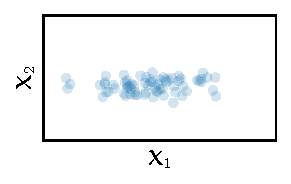
\includegraphics[height=.3\textheight]{figures/generated/pca/cloud_aligned.pdf}
\end{center}
\vspace{-20pt}
\end{block}
\begin{block}{Data low-dimensional but no feature can be dropped:}
\begin{center}
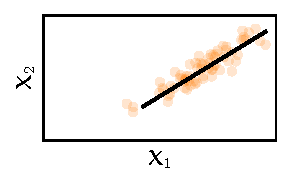
\includegraphics[height=.3\textheight]{figures/generated/pca/cloud_not_aligned.pdf}
\end{center}

Find a better referential in which to represent the data
\end{block}
\end{frame}
\begin{frame}[label={sec:org4374e8f}]{Linear regression: projection on the column space of \(X\)}
\begin{structureenv} %% top
\begin{columns}
\begin{column}{.3\columnwidth}
\begin{equation}
\hat{\y} = \X \, \hat{\bbeta}
\end{equation}
\end{column}

\begin{column}{.7\columnwidth}
\vspace{-17pt}
\begin{center}
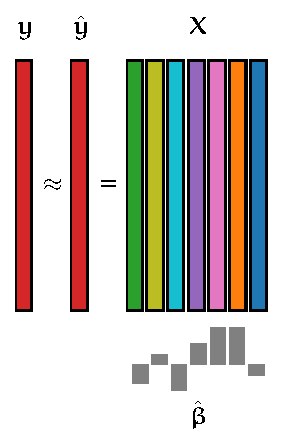
\includegraphics[height=.7\textheight]{figures/generated/dim_reduction_colors/regression_full_3.pdf}
\end{center}
\end{column}
\end{columns}
\end{structureenv}

\begin{structureenv} %% bottom
\begin{itemize}
\item Too many features: high variance \& unstable solution
\item Feature selection: drop some columns of \(\X\)
\item Other ways to build a family of \(k\) vectors on which to regress \(\y\)?
\end{itemize}
\end{structureenv}
\end{frame}
\begin{frame}[label={sec:orgdd74719}]{Linear decomposition: low-rank approximation of \(\X\)}
Minimize
\begin{equation}
\| \X - \W \, \bH \|_{\F}^2 = \sum_{i, j} ( \X_{i,j} - (\W \, \bH)_{i,j})^2
\end{equation}
\begin{center}
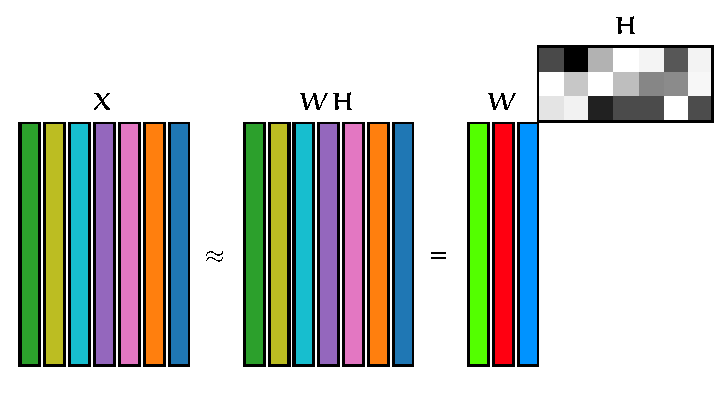
\includegraphics[height=.5\textheight]{figures/generated/dim_reduction_colors/factorization_3.pdf}
\end{center}
\end{frame}
\begin{frame}[label={sec:org9975e14}]{Linear regression after dimensionality reduction}
\begin{equation}
\hat{\y} = \W \, \hat{\bbeta}
\end{equation}
\begin{center}
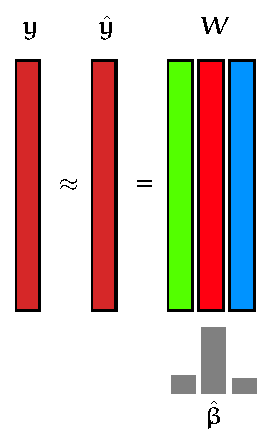
\includegraphics[height=.7\textheight]{figures/generated/dim_reduction_colors/regression_reduced_3.pdf}
\end{center}
\end{frame}
\begin{frame}[label={sec:org3307e6a}]{Prediction for a new data point \(\x \in \R^{p}\)}
\begin{itemize}
\item Find the combination of rows of \(\bH\) that is closest to \(\x\): regress \(\x\) on \(\bH^T\)
\item Multiply by \(\hat{\bbeta}\)
\end{itemize}
    \begin{equation}
\x \in \R^p \rightarrow \text{projection} \rightarrow \mathbold{w} \in \R^k \rightarrow \langle \cdot \, , \, \hat{\bbeta}\rangle \rightarrow \hat{y} \in \R
    \end{equation}
\end{frame}
\begin{frame}[label={sec:org1ef63b0}]{Principal Component Analysis}
\begin{itemize}
\item Singular Value Decomposition of \(\X\):
\end{itemize}
\begin{equation}
\X = \U \, \bS \, \V^T
\end{equation}
with \(\X \in \R^{n \times p}\), \(\U \in \R^{n \times r}\), \(\bS \in \R^{r \times r}\), \(\V \in \R^{r \times p}\)
\begin{itemize}
\item \(r = \min(n, p)\)
\item \(\bS \succeq 0\) diagonal with decreasing values \(s_j\) along the diagonal
\item \(\U^T\, \U = I_r\)
\item \(\V^T\, \V = I_r\)
\end{itemize}

Truncating the SVD to keep only the first \(k\) components gives the best rank-\(k\) approximation of \(\X\)
\begin{center}
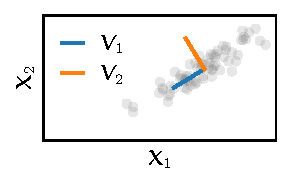
\includegraphics[height=.3\textheight]{figures/generated/pca/cloud_not_aligned_with_pc.pdf}
\end{center}
\end{frame}
\begin{frame}[label={sec:org281ec0a}]{Singular Value Decomposition}
\begin{equation}
\X = \U \, \bS \, \V^T
\end{equation}
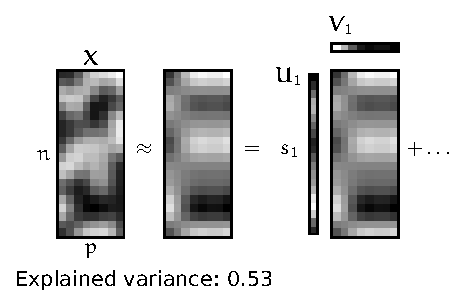
\includegraphics[height=.5 \textheight]{figures/generated/pca_step_by_step/pca_steps_1.pdf}

\begin{equation}
\U^T \, \U = I_p
\end{equation}
\begin{equation}
\V^T \, \V = I_p
\end{equation}
\end{frame}

\begin{frame}[label={sec:orgcd77dfe}]{Singular Value Decomposition}
\begin{equation}
\X = \U \, \bS \, \V^T
\end{equation}
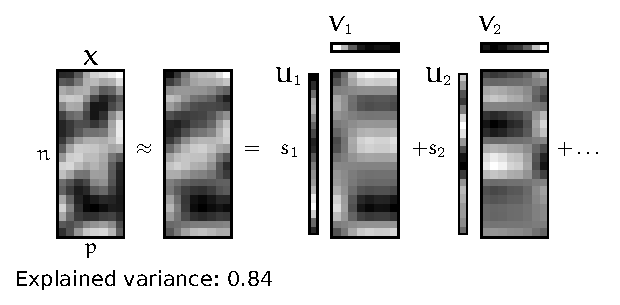
\includegraphics[height=.5 \textheight]{figures/generated/pca_step_by_step/pca_steps_2.pdf}

\begin{equation}
\U^T \, \U = I_p
\end{equation}
\begin{equation}
\V^T \, \V = I_p
\end{equation}
\end{frame}


\begin{frame}[label={sec:org7c6be3d}]{Singular Value Decomposition}
\begin{equation}
\X = \U \, \bS \, \V^T
\end{equation}
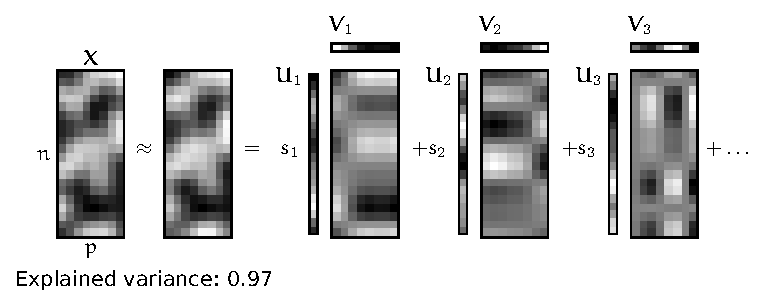
\includegraphics[height=.5 \textheight]{figures/generated/pca_step_by_step/pca_steps_3.pdf}

\begin{equation}
\U^T \, \U = I_p
\end{equation}
\begin{equation}
\V^T \, \V = I_p
\end{equation}
\end{frame}

\begin{frame}[label={sec:org463c63d}]{Other decomposition methods}
Many other methods use the same objective (sum of squared reconstruction errors), but add penalties or constraints on the factors
\begin{itemize}
\item Dictionary Learning
\item Non-negative Matrix Factorization
\item K-means clustering
\item \ldots{}
\end{itemize}

\begin{block}{What about \(\y\)?}
\begin{itemize}
\item PCA is an example of \emph{unsupervised} learning: it does not use \(\y\)
\item Some other methods take it into account: \eg Partial Least Squares
\end{itemize}
\end{block}
\end{frame}
\begin{frame}[label={sec:org516564f}]{Ridge regression and PCA}
\begin{itemize}
\item Both ridge regression and PC regression compute the coordinates of \(\y\) in the basis given by the SVD of \(\X\)
\item Ridge shrinks the coordinate along \(\U_j\) by a factor \(s_j^2 / (s_j^2 + \alpha)\)
\item PC regression sets the coordinates to 0 except for those corresponding to the \(k\) largest \(s_j\): shrinks by a factor \(\mathbold{1}_{\{j \leq k\}}\)
\end{itemize}

\begin{center}
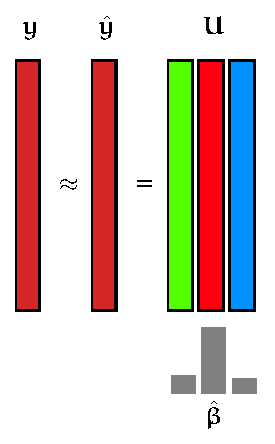
\includegraphics[height=.6\textheight]{figures/generated/dim_reduction_colors/regression_reduced_3_svd.pdf}
\end{center}
\end{frame}
\section{Conclusion: summary of pitfalls}
\label{sec:org7a22ec1}
\begin{frame}[label={sec:org4ee209f}]{Split choice example: time series}
Don't ignore dependencies between samples: which is easier?
\begin{center}
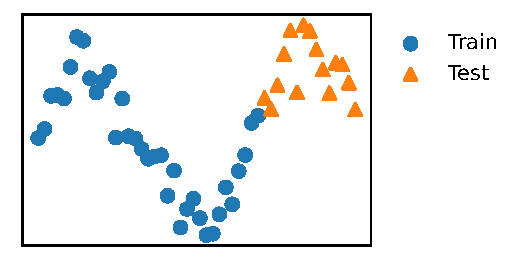
\includegraphics[height=.3 \textheight]{figures/generated/time_series_cv/kfold.pdf}
\end{center}

\begin{center}
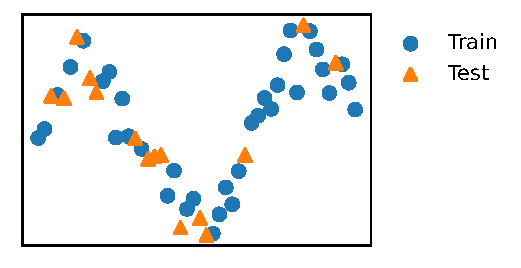
\includegraphics[height=.3 \textheight]{figures/generated/time_series_cv/kfold_shuffled.pdf}
\end{center}

Use the appropriate \href{https://scikit-learn.org/stable/modules/cross\_validation.html\#cross-validation-iterators}{cross-validation iterator}
\end{frame}
\begin{frame}[label={sec:orgcf322d9}]{Remember that CV training sets overlap}
\begin{center}
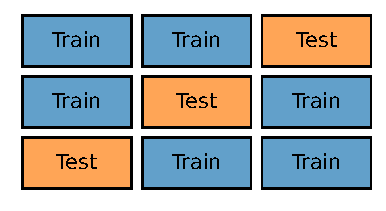
\includegraphics[height=.6 \textheight]{figures/generated/train_eval_test/cv_not_nested.pdf}
\end{center}

So the scores are not independent! Their variance can be underestimated.
\end{frame}

\begin{frame}[label={sec:org6f9bf11},fragile]{Some pitfalls with cross-validation}
 \small
\begin{block}{Overfitting the hyperparameters}
\begin{itemize}
\item select hyperparameters with nested CV \href{https://scikit-learn.org/stable/modules/generated/sklearn.model\_selection.GridSearchCV.html}{\texttt{sklearn.model\_selection.GridSearchCV}}
\end{itemize}
\end{block}
\begin{block}{Fitting part of the pipeline on the whole dataset}
\begin{itemize}
\item use  \href{https://scikit-learn.org/stable/modules/generated/sklearn.pipeline.Pipeline.html}{\texttt{sklearn.pipeline.Pipeline}}
\end{itemize}
\end{block}
\begin{block}{Ignoring dependencies between samples}
\begin{itemize}
\item e.g. time series: use appropriate \href{https://scikit-learn.org/stable/modules/cross\_validation.html\#cross-validation-iterators}{cross-validation iterator}
\end{itemize}
\end{block}
\begin{block}{Ignoring dependencies between CV scores}
\begin{itemize}
\item Training sets overlap: cross-validation scores of different splits are not independent
\end{itemize}
\end{block}
\begin{block}{Over-interpreting good CV scores}
\end{block}
\end{frame}
\end{document}